{\small
\section{Objektorientierung}

\subsection{Klassen und Objekte}{\label{Klassen}}
    Klassen bestehen aus \textbf{Variablen} und \textbf{Methoden}.\\
    Objekte können aus Klassen erzeugt werden: \verb|Point a = new Point()|\\
    Konstruktoren können in den meisten IDEs automatisch generiert werden.

    Sofern kein Konstruktor definiert ist, wird der \textbf{Default-Konstruktor} verwendet. Die Instanzvariablen werden mit
    Default-Werten initialisiert (primitive mit \verb|0|, Referenzdatentypen mit \verb|NULL|)\\

    Klassen arbeiten mit Referenzen, dies muss bei Zuweisungen beachtet werden:
    \begin{center}
        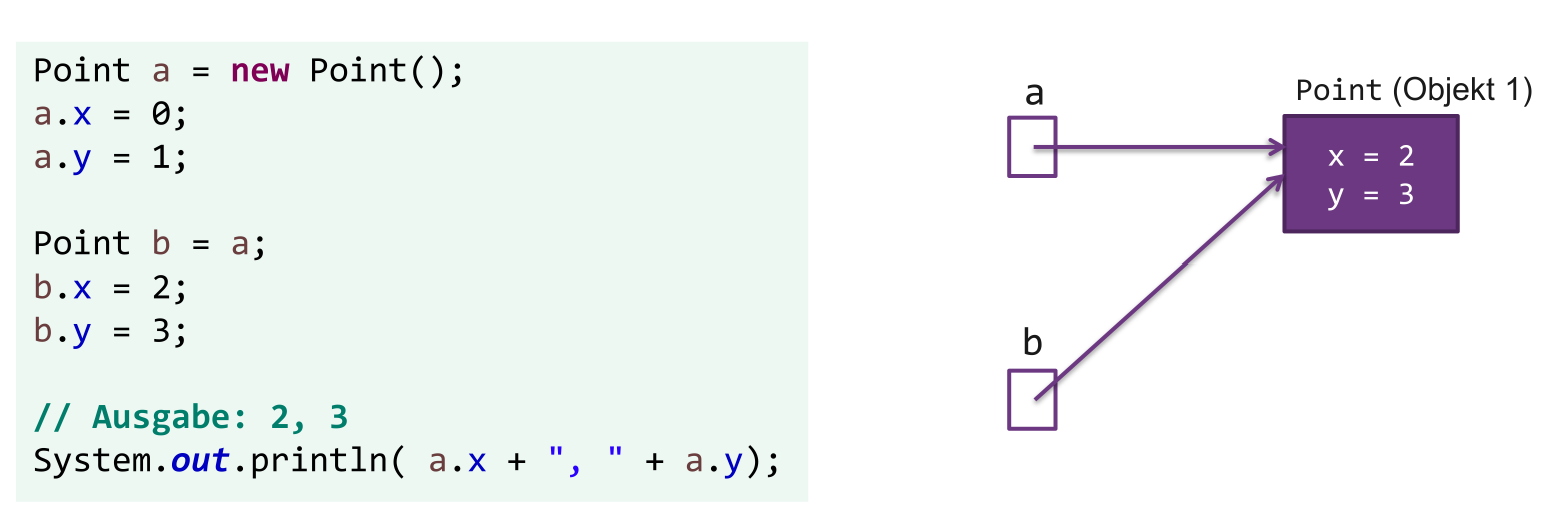
\includegraphics[width=0.9\columnwidth]{pictures/copy-semantics.png}    
    \end{center}
    \vspace{-0.3cm}

\subsection{Methoden}

    \subsubsection{Parameter}
        Java verwendet \textit{immer} \textbf{Call by Value}. Die Argumente werden kopiert und als Parameter übergeben. Dies kann zu unterschiedlichem Verhalten
        je nach Datentyp führen:\\

        \textbf{Primitive Datentypen}:\\
        Methode arbeitet mit Kopie des Wertes
        \begin{center}
            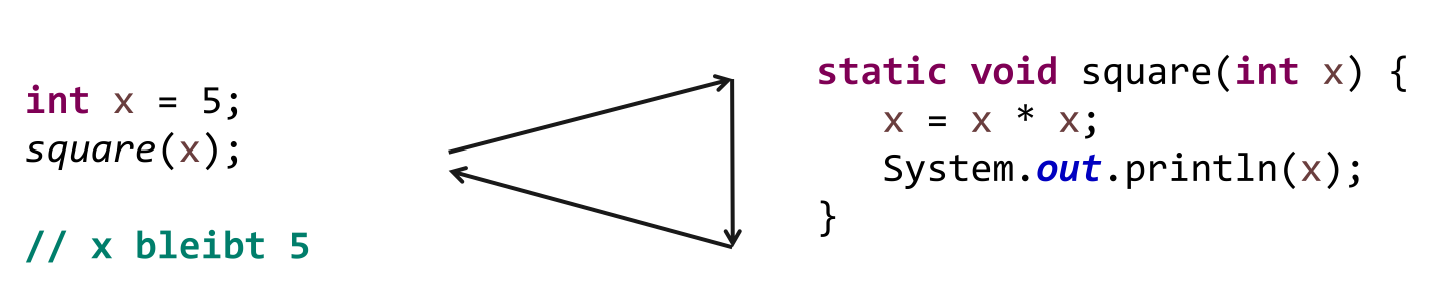
\includegraphics[width=0.9\columnwidth]{pictures/primitive-params.png}    
        \end{center}

        \textbf{Referenzdatentypen}:\\
        Methode arbeitet mit Kopie der Referenz
        \begin{center}
            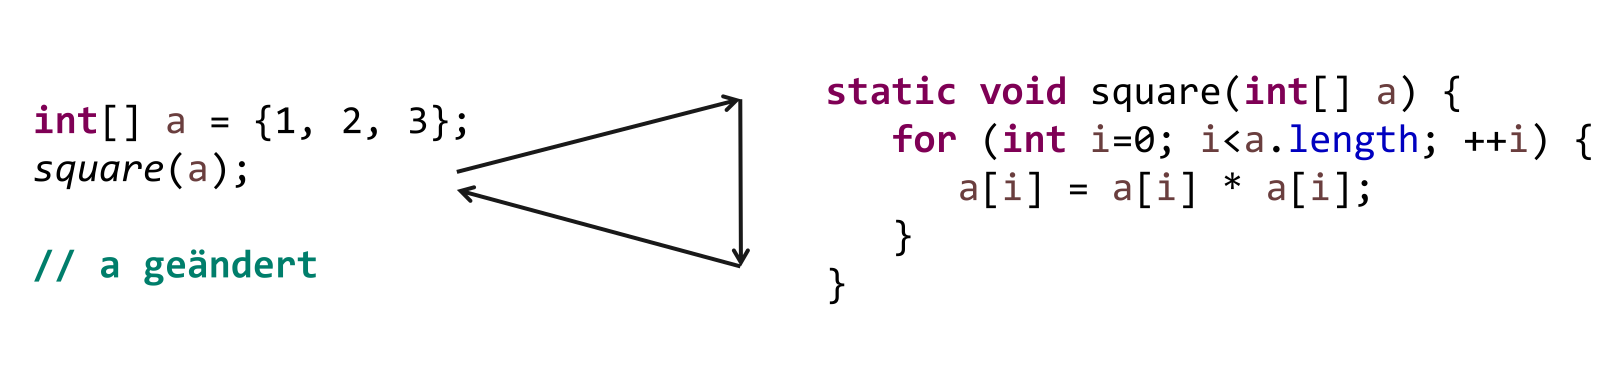
\includegraphics[width=0.9\columnwidth]{pictures/reference-params.png}    
        \end{center}
        \vspace{-0.3cm} 

    \subsubsection{Variadische Methoden}
        Falls bei Funktionen die Anzahl der Argumente nicht im Voraus bekannt ist, kann folgende
        Syntax verwendet werden: \verb|static int sum(int... numbers){}|\\
        Der Compiler generiert ein Array aus der Parameterliste.
        \vspace{-0.2cm}

\subsection{Methodenreferenzen}
    Anstatt Hilfsklassen für häufig verwendete Methoden zu erstellen, kann auch mit 
    Methodenreferenzen gearbeitet werden, wie in C++ mit Funktionszeigern. Für die Referenzierung braucht es
    eine Funktionsschnittstelle und die Implementierung. Methodenreferenzen benötigen eine aufrufende \textbf{höherwertige} Funktion. \\
    Referenz-Varianten:\\
    \begin{tabular}{ll}
        \verb|this::compare|    & Methode \verb|compare| im selben Objekt \\
        \verb|other::compare|   & Methode \verb|compare| in Objekt \textit{other} \\
        \verb|MyClass::compare| & Statische Methode in \textit{MyClass} \\
        \verb|MyClass::new|     & Konstruktor der Klasse \textit{MyClass} \\
    \end{tabular}
    \vspace{-0.1cm} 

    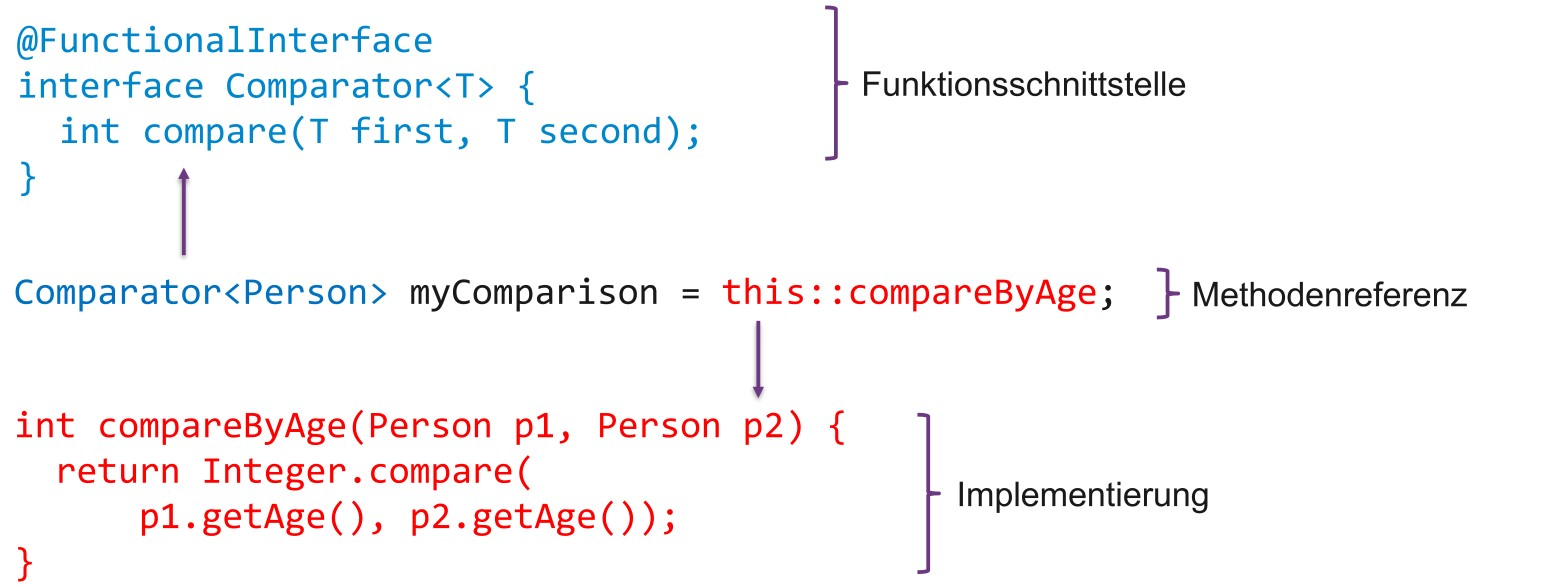
\includegraphics[width=\linewidth]{pictures/methoden-referenzen.jpg}
    \vspace{-0.2cm} 


    \subsubsection{Lambdas $\qquad \qquad$ $\sim$ 3 Zeilen $\rightarrow$ sonst: siehe auch \ref{Lambdas}}
        Ad-Hoc Implementierung anstatt einer expliziten Methodenreferenz. \\
        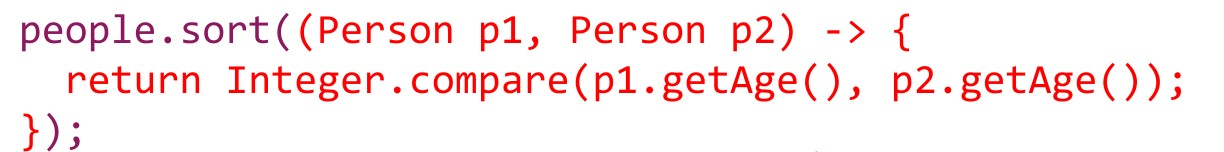
\includegraphics[width=\linewidth-2cm]{pictures/lambda.jpg} \\
        \verb|Person|,\verb|{}| und \verb|return| sind optional, wenn nur ein Ausdruck enthalten
        \vspace{-0.1cm} 

\subsection{Unit Testing: Siehe auch Kapitel \ref{Unit-Test}}
    Unit Testing ist eine der Varianten, um Bugs zu verhindern. In guten Unit Tests sollen möglichst alle relevanten Fälle abgedeckt sein.
    Dazu gehören Standardfälle (im Bereich der Funktion, auch \textbf{Äquivalenzklassen} genannt) und Edge Cases (z.B. 0, max. und min. Bereich, usw.).\\
    \vspace{-0.3cm}

    \begin{tabular}{l l}
        $\bullet$ Pro Klasse eine Test-Klasse & $\bullet$ Pro Testfall eine Methode\\
    \end{tabular}
    \vspace{-0.3cm}

    \subsubsection{Assert-Methoden}
        \begin{center}
            \begin{tabular}{ll}
                \rowcolor[RGB]{239,239,239} 
                \textbf{Methode} & \textbf{Bedingung} \\ \hline
                assertEquals(expected, actual) & für prim. und Referenztypen \\
                assertNotEquals(expected, actual) & \\
                assertSame(expected, actual) & actual == expected\\
                assertNotSame(expected, actual) & actual != expected\\
                assertTrue(condition) & condition\\
                assertFalse(condition) & !condition\\
                assertNull(value) & value == null\\
                assertNotNull(value) & value != null\\
            \end{tabular}
        \end{center}
        \vspace{-0.5cm}

    \begin{center}
        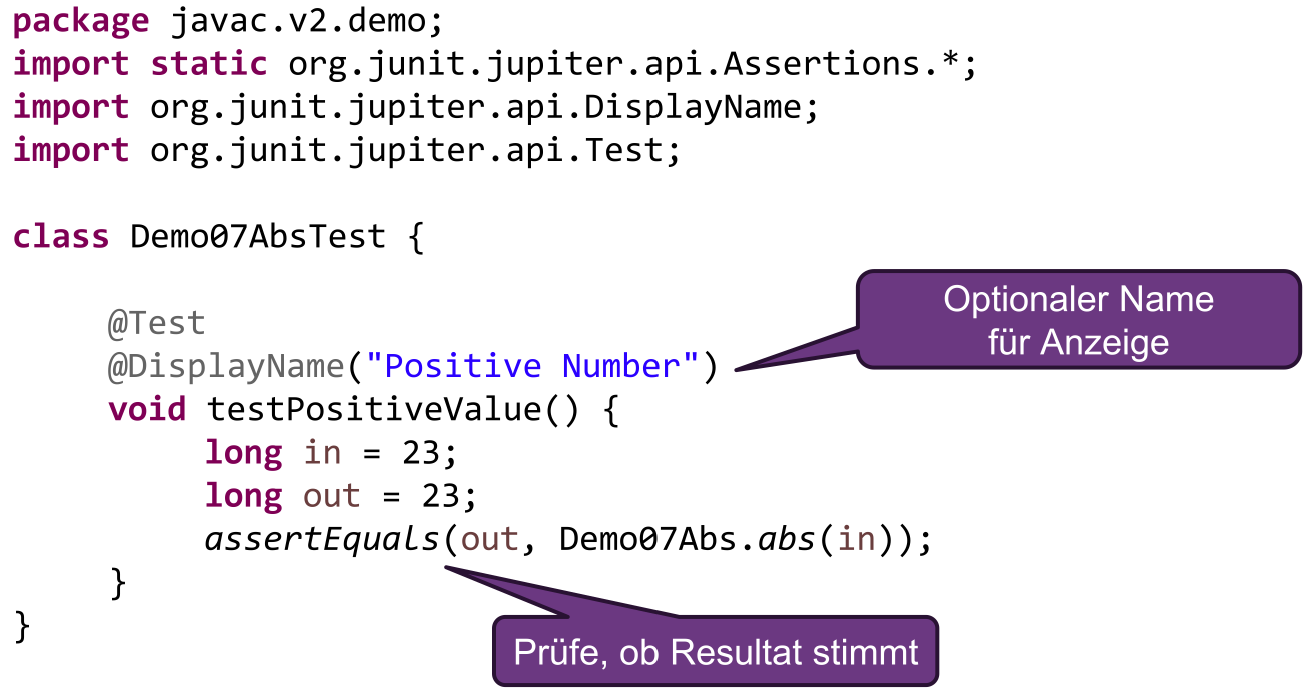
\includegraphics[width=0.8\columnwidth]{pictures/testmethode.png}    
    \end{center}
    \vspace{-0.4cm} 

    \subsubsection{Sichtbarkeit}
        \vspace{-0.1cm}
        \begin{center}
            \begin{tabular}{ll}
                \rowcolor[RGB]{239,239,239} 
                \textbf{Keyword} & \textbf{Sichtbar für} \\ \hline
                public & Alle Klassen \\
                protected & Klassen im selben Package und abg. Klassen\\
                (keines) & Klassen im selben Package \\
                private & Nur eigene Klasse \\
            \end{tabular}
        \end{center}
        \vspace{-0.2cm}

        Für Zugriffe auf \verb|private|-Variablen können Getter- und Setter-Methoden definiert werden. Siehe auch \ref{GetSet}
        \vspace{-0.1cm} 


\subsection{Generics $\rightarrow$ typ-unabhängige Frames erstellen}
    
    {\small \textit{Nicht enthalten: Typebounds, Wildcardtypen, Covarianz, Type-Erasure}}
    \vspace{-0.1cm} 

    \subsubsection{Generische Variablen}
        Die Variable dient als Platzhalter innerhalb einer generischen Klasse, Methode oder Interface. Sie wird mit \verb|<>| umschlossen 
        und kann innerhalb der Klasse,... wie ein normaler Typ verwendet werden.\\
        Häufig verwendete Namen:\\
        \begin{tabular}{l l|l l}\hline
            E & Element & T & Type\\
            K & Key     & V & Value\\
            N & Number  & S, U ,V,... & 2ter, 3ter, 4ter Type \\\hline
        \end{tabular}\\
        \\
        Mehrere Typ-Variablen gleichzeitig sind zulässig, z.B. \verb|<T, U>|
        \vspace{-0.1cm}

    \subsubsection{Generische Klassen}
        Klasse mit Typ-Variable (Platzhalter für unbekannten Typ).\\
        Verschachtelung bei der Anwendung ist zulässig.\\
        \vspace{-0.1cm}
        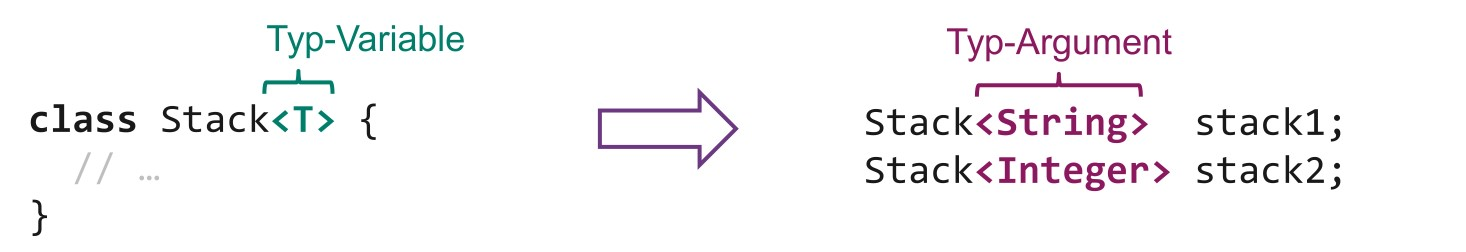
\includegraphics[width=0.8\linewidth]{pictures/generic-class.jpg}\\
        Bei der Anwendung macht der Compiler eine statische Prüfung des Datentyps. der Type-Cast entfällt (auto-boxing, -unboxing)
        \vspace{-0.1cm}


    \subsubsection{Generische Interfaces}\label{StackIterator}
        Gleiche Syntaxregeln wie bei generischen Klassen, jede Klasse kann generische Interfaces implementieren.\\
        Anwendung:\\
        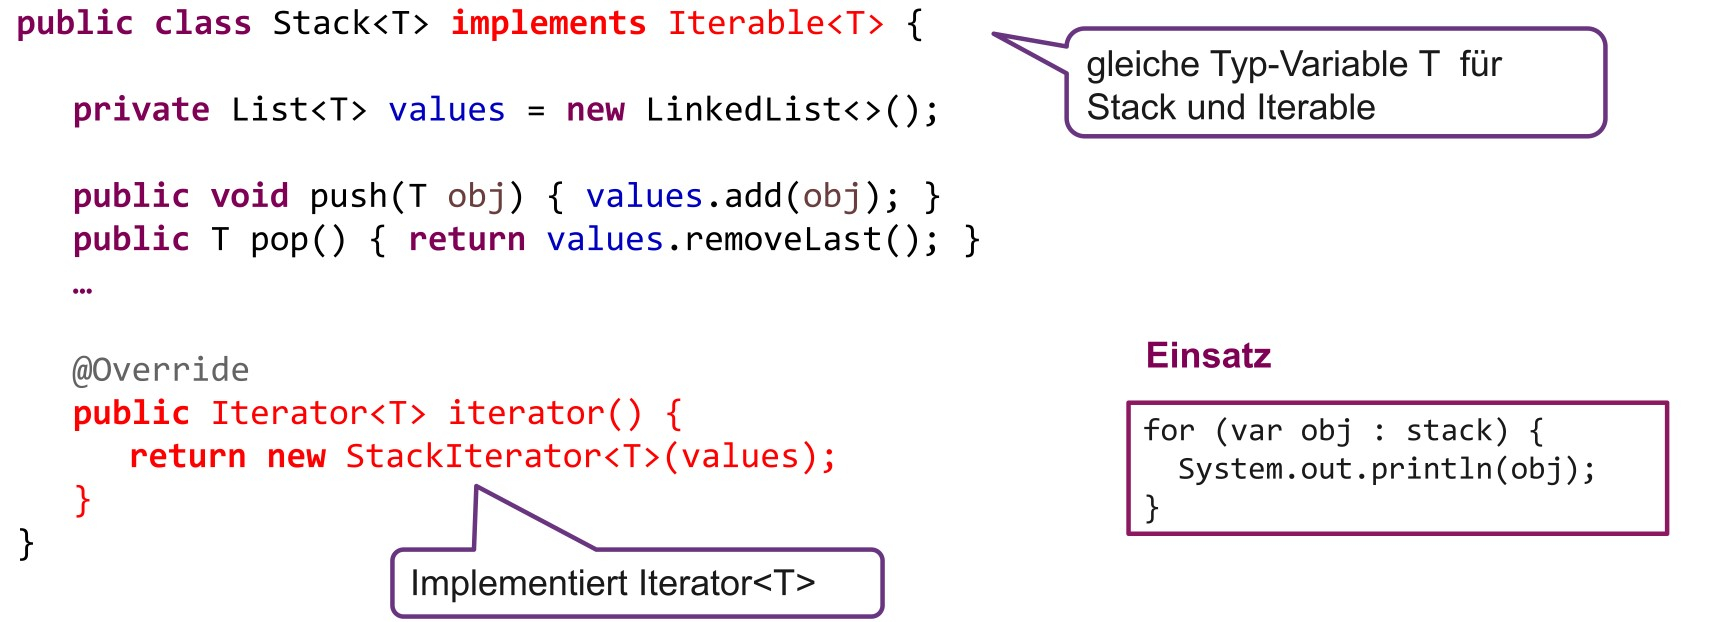
\includegraphics[width=0.8\linewidth]{pictures/generic-interface1.jpg}
        % \hrule
        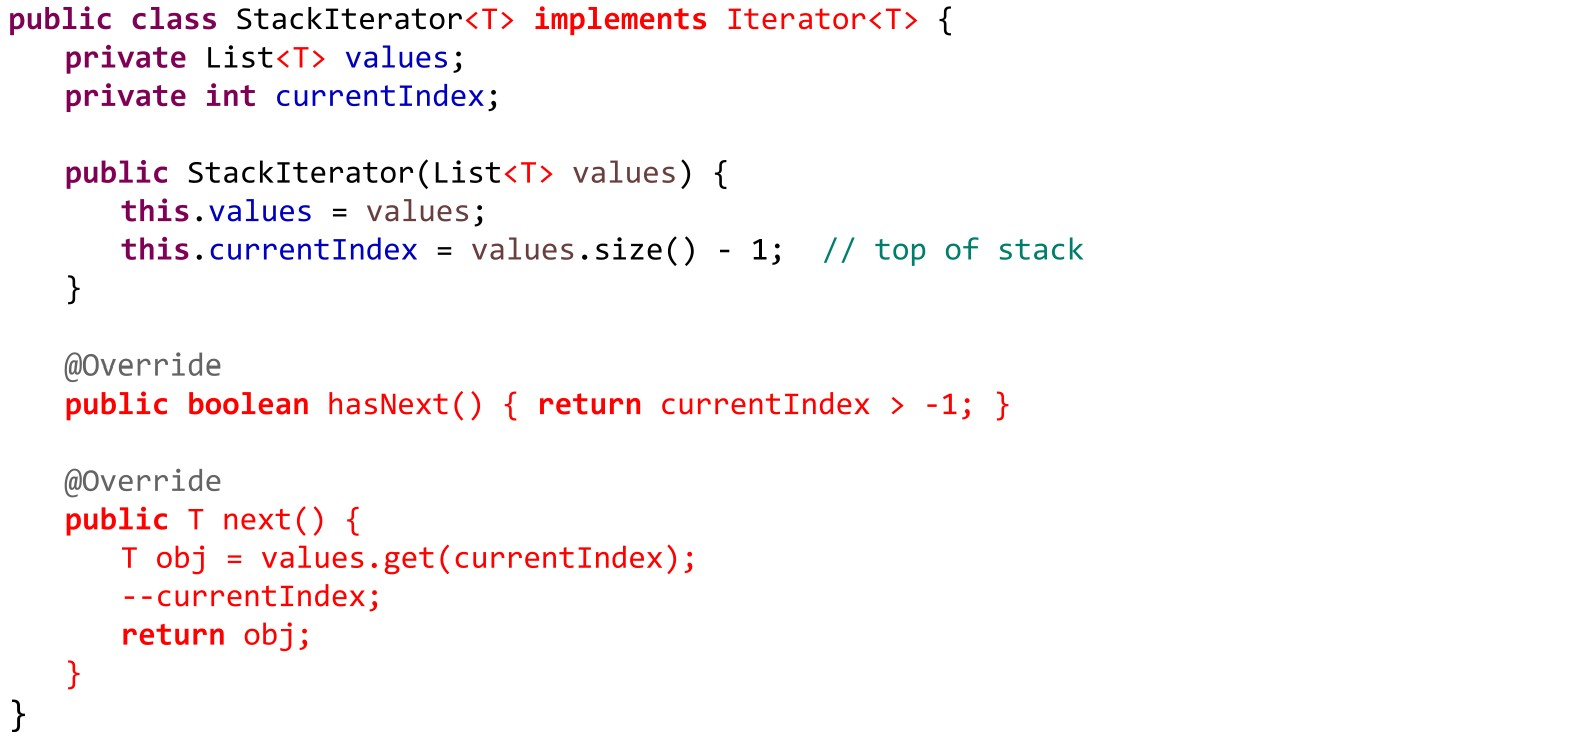
\includegraphics[width=0.8\linewidth]{pictures/generic-interface2.jpg}
        \vspace{-0.1cm}

    \subsubsection{Generische Methoden}
        \begin{tabular}{l l}
            $\bullet$ & unabhängig von generischen Klassen und Interfaces\\
            $\bullet$ & Implementation kann in normalen, nicht generischen Klassen\\
                    & erfolgen und ist auch in statischen Methoden zulässig.\\
        \end{tabular}

        Die Typ-Variable muss in Klammer \verb|<>| vor dem Rückgabewert stehen. \\
        \verb|public static <T> List<T> merge(List<T> a, List<T> b) { … }|

}